%! TEX root = 0-main.tex
\chapter{Multi-particle Systems}
In the appendix, we discuss three-particle systems. This discussion is extended to a system of \(n\) particles. There are two cases we can consider: the discrete case and the continuous case. As it is impossible to describe the exact motion, we instead focus on statistical properties of these systems.
\section{Properties}
\subsection{Linear Momentum}
The center of mass of a system is the mass-weighted average of the positions in the system. For a discrete system, this is given by
\begin{equation}
	\vv{R}_{cm} = \frac{\sum_\alpha m_\alpha \vv r_\alpha}{\sum_\alpha m_\alpha}
\end{equation}
while for the continuous case, it is given
\begin{equation}
	\vv{R}_{cm}=  \frac{\int\vv{r}\d{m}}{\int\d{m}}=\frac{1}{M}\int r \rho\d\tau
\end{equation}
For a 3-body system, we saw that the internal interactions cancelled out and did not affect the centre of mass. However, forces due to an external force can have such an effect. This is true of the \(N\)-body system as well. The internal force on particle \(\alpha\) can be written as
\[\vv f_\alpha = \sum_{\beta\neq\alpha} f_{\alpha\beta}\]
The total force on a particle is then
\[\vv F_\alpha = \vv f_\alpha + \vv f_\alpha^{ext} = \dot{\vv p}_\alpha\]
The total force on every particle is then given
\[\vv{F}^{tot} = \sum_{\alpha}\vv F_\alpha  = \sum_{\alpha,\beta\neq\alpha} \vv f_{\alpha\beta} + \sum_\alpha \vv f_\alpha^{ext}\]
By newton's third law, we have \(f_{\alpha\beta}=-f_{\beta\alpha}\), so the total force reduces to
\begin{equation}
	\vv F^{tot} = \sum_\alpha \vv f_\alpha^{ext}
\end{equation}
or, the total force on a system is that applied to it by external forces. Further, we have
\[\vv F^{tot} = \dot{\vv p}^{tot} = \sum_\alpha\dot{\vv p}_\alpha = \sum_\alpha m_\alpha\ddot{\vv r}_\alpha = \der{}{t2}\sum_\alpha m_\alpha \vv r_\alpha = \der{}{t2}M\vv{R}_{cm}\]
or, the centre of mass behaves like a single particle with mass \(M = \sum_\alpha m_\alpha\) acted upon by the sum of all external forces. 
\[\vv F^{tot} = M\ddot{\vv R}_{cm}\]
The total linear momentum of the system further is the same as that of a single particle of mass \(M\) located at the centre of mass. 
\[\vv p^{tot} = \sum_\alpha m_\alpha \dot{\vv r}_\alpha = \der{}{t}\sum_\alpha m_\alpha \vv r_\alpha = M\dot{\vv R}_{cm}\]
Thus, in the absense of foreces, the total linear momentum of a system is equal to the linear momentum of the cenre of mass.
\[\dot{\vv p}^{tot} = \vv{F}^{tot} = 0\]
\subsection{Angular Momentum}
Similar results may be obtained for the angular momentum of a system, keeping in mind that the angular momentum depends on the choice of origin. We provide all particles a vector \(\vv{r}_{\alpha}'\) such that the positions of each particles \(\vv r_\alpha\) may be specified:
\[\vv r_\alpha = \vv{R}_{cm}+\vv r_\alpha'\]
Computing the angular momentum about the orgin, we have
\[\vv L_\alpha = \vv r_\alpha \times \vv p_\alpha\]
and total angular momentum
\[\vv L^{tot} = \sum_\alpha\vv L_\alpha = \sum_\alpha \vv r_\alpha ' \times m_\alpha \dot{\vv r}_\alpha=\sum_\alpha m_\alpha\left(\vv{R}_{cm}+\vv{r}_\alpha ' \right)\times\left(\dot{\vv R}_{cm}+\dot{\vv r '}_\alpha\right)\]
Expanding,
\[\vv L^{tot} = \sum_\alpha m_\alpha\left(\vv{R}_{cm}\times \dot{\vv R}_{cm} + \vv{r}'_\alpha\times\dot{\vv R}_{cm} + \vv{R}_{cm}\times \dot{\vv r'}_\alpha + \vv{r}'_\alpha\times\dot{\vv r'}_\alpha\right)\]
Using the bilinearity of the cross product, the second term may be rewritten
\[\left(\sum_\alpha m_\alpha \vv{r}'_\alpha\right)\times\dot{\vv R}_{cm} = \sum_\alpha m_\alpha \left(\vv r_\alpha - \vv R_{cm}\right)\times \dot{\vv R}_{cm}=\left(M\vv R_{cm}-M\vv R_{cm}\right)\times \dot{\vv R}_{cm}=0\]
This similarly applies to the third term. Thus,
\[\vv{L}^{tot} = M\vv{R}_{cm}\times\dot{\vv R}_cm+ \sum_\alpha m_\alpha \vv{r}'_\alpha\times\dot{\vv r'}_\alpha\]
or the total angular momentum can be written as the angular momentum of the centre of mass added to the angular momentum of the particles around the centre of mass
\begin{equation}
	\vv{L}^{tot} = \vv{L}_{cm} + \sum_\alpha \vv{L}'_\alpha
\end{equation}
\subsection{Moment of Inertia}
If instead of a discrete system of particles, we consider a rigid, continous body, the individual angular momenta can no longar point in an arbitrary direction; all angular momenta must be parallel. Considering an infinitessimal mass \(\d{m}\) with displacement \(\vv{r}'_\alpha\) from the center of mass with angle \(\theta_\alpha\) to the angular frequency vector \(\vv\omega\), the velocity can be written
\[\dot {\vv r'}_\alpha = \omega\times \vv{r}'_\alpha=\omega r_\alpha ' \sin(\theta_\alpha)\hat \phi_\alpha\]
Summing the total angular momentum
\[\sum_\alpha \vv L'_\alpha = \sum_\alpha m_\alpha \vv r_\alpha ' \times \left(\vv\omega \times \vv r'_\alpha\right) = \omega \sum_\alpha m_\alpha r_\alpha ' \sin\theta_\alpha \left(\vv{r}_\alpha ' \times\hat \phi_\alpha\right)\]
If we restrict our consideration of the angular momentum parallel to the rotation,
\[L_\parallel = \omega\sum_\alpha m_\alpha r_\alpha ' \sin\theta_\alpha \hat\omega * \left(\vv r'_\alpha \times \hat\phi_\alpha\right)\]
Using the cyclic property of the scalar triple product, we can rewrite it as \(\hat\phi_\alpha * \left(\hat\omega \times \vv r'_\alpha\right) = \hat\phi_\alpha * (r'_\alpha\sin\theta_\alpha\hat\phi_\alpha) = r'\sin\theta_\alpha\)
so the parallel component of the angular momentum can be written
\[L_\parallel = \omega\sum_\alpha m_\alpha r_\alpha'^2 \sin^2\theta_\alpha\]
\begin{equation}
	L_\parallel = \omega\sum_\alpha m_\alpha r_{\alpha,\perp}'^2
\end{equation}
or, for a continuous distribution,
\begin{equation}
	L_\parallel = \omega \int r_{\alpha,\perp}'^2\d{m}
\end{equation}

Interestingly, \(\vv{L}\) need not be parallel to the rotation \(\vv{\omega}\). As an example, we consider two particle restricted to motion on two parallel circular tracks. The angular momentum goes through the centres of these tracks, perpendicular to the surfaces. If we take \(m_1\) to be opposite \(m_2\), the angular momentum is actually at an angle to the rotation \(\vv\omega\). 
\begin{center}
	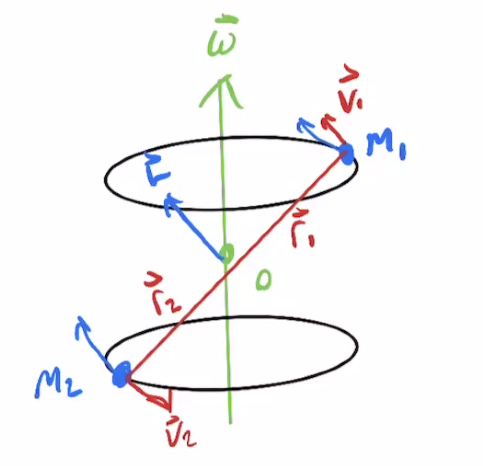
\includegraphics[scale = 0.4]{lwcounter.png}
\end{center}

We recognize
\begin{equation}
	L_\parallel = \omega I
\end{equation}
as the definition of the moment of inertia.

\subsection{Torque}
The torque on an individual particle is defined to be:
\begin{equation}
	\vv{N}_\alpha = \dot{\vv L}_\alpha = \vv r_\alpha \times \vv F_\alpha
\end{equation}
This can be written more verbosely as
\[\vv N_\alpha = \vv r_\alpha \vv{f}_\alpha^{ext} + \vv r_\alpha\times \vv f_\alpha\]
as the sum of the internal and external torques.
\[\vv{N}^{tot} = \sum_\alpha \vv{N}_\alpha = \sum_\alpha \vv{N}_\alpha^{ext} + \sum_\alpha\vv r_\alpha\times \left(\sum_{\beta \neq \alpha} \vv f_{\alpha\beta}\right)\]
We can once again rewrite the last term as
\[\sum_\alpha\sum_{\beta>\alpha} \left(\vv r_\alpha \times\vv f_{\alpha\beta}+\vv r_\beta \times \vv f_{\beta\alpha}\right)=0\]
which follows from the ``strong'' Newton's third law.\footnote{The ``weak'' Newton's third law only states that \(f_{\alpha\beta} = -f_{\beta\alpha}\) and may be false}, This law states that for central forces, 
\[\vv f_{\alpha\beta} = f_{\alpha\beta} \left(\vv r_\alpha- \vv r_{\beta}\right)\]
Thus,
\begin{equation}
	\vv{N}^{tot} = \sum_\alpha \vv N_\alpha^{ext}
\end{equation}

Additionally, we can relate the torque to the angular momentum as follows:
\[\der{L}{t} = m\vv{v}\times\vv{v}+\vv r\times\der{\vv p}{t} = \vv \tau\]

\subsection{Kinetic Energy}
For an arbitrary collection of particles, the work done one a particle \(\alpha\) between time \(t_1,t_2\) is
\[W_{12\alpha} = \int_1^2\vv F_\alpha*\d{\vv r_\alpha} = \int_1^2M_\alpha\ddot{\vv{r}}_{\alpha}*\dot{\vv r}_\alpha\d{t} = \int_1^2m_\alpha \frac{1}{2}\der{}{t}\dot r^2_\alpha\d{t}=\int_1^2\d{T_\alpha}\]
Thus, for the total system,
\[W_{12}^{tot} = \sum_\alpha\int_1^2\d{T_\alpha}= \Delta T^{tot}\]
where
\[T^{tot} = \sum_\alpha \frac{1}{2}m_\alpha \dot r_\alpha^2\]
Transforming to \(\vv r_\alpha = \vv R_{cm} + \vv{r}'_\alpha\), we obtain
\[T^{tot} = \sum_\alpha \frac{1}{2}m_\alpha \dot r'^2_\alpha + \frac{1}{2}m_\alpha\dot R_{cm}^2+m_\alpha \dot {\vv R}_{cm}*\dot{\vv r'}\]
however, we know that \(\sum m_\alpha \dot{\vv r'}_\alpha =\der{}{t}\sum_\alpha\vv r'_\alpha = \der{}{t}0 = 0\), so
\begin{equation}
	T^{tot} = \frac{1}{2}M\dot R_{cm}^2+\sum_\alpha \frac{1}{2}m_\alpha \dot r'^2_\alpha
\end{equation}
or, the kinetic energy is the sum of the internal kinetic energy, and the tranlational kinetic energy of the system

\subsubsection{Rotating Rigid Body}
If we imagine a rigid body rotating around an axis with \(\vv\omega\). We can write the kinetic energy wrt to a point along the axis of rotation
\begin{align*}
	T&=\frac{1}{2}\int v^2\d{m}\\
	 &=\frac{1}{2}\iiint \rho(r) v^2(r)\d[3]r\\
	 &=\frac{1}{2}\iiint \rho r^2_\perp \omega^2\d[3]r\\
	 &=\frac{1}{2}\left(\iiint \rho r^2_\perp\d[3]r\right)\omega^2\\
	 &=\frac{1}{2}I\omega^2
\end{align*}
If we instead choose the kinetic energy in terms of the centre of mass, we obtain
\[T = \frac{1}{2} MV_{cm}^2 + \sum_{\alpha}\frac{1}{2}m_\alpha v_\alpha'^2\]
Using \(v' = \abs{\vv \omega\times \vv r'} = \omega r_\perp '\) we see that this becomes
\[T = \frac{1}{2}MV_{cm}^2+\frac{1}{2}I'\omega^2\]
if \(D\) is the distance to the centre of mass from the axis of rotation, we obtain \(V_{cm} = \abs{\vv\omega\times\vv D} = \omega D\), so
\[T = \frac{1}{2}MD^2 \omega^2+\frac{1}{2}I'\omega^2\]
and thus we recover the \emph{parallel axis theorem}
\begin{equation}
	I' = MD^2+I_{cm}
\end{equation}

\section{Scattering and Collisions}
A particle 1 is shot at a stationary particle 2, albeit with a vertical displacement \(b\), called the \emph{impact parameter}. The particles start at infinity, and end at infinity. We are interested in the deflection angle \(\phi\) between the initial velocity of particle 1 \(\vv{u_1}\) and the final velocity of \(\vv v_2\). The second particle starts at rest and leaves with velocity \(\vv v_2\) at angle \(\xi\). 

Transforming to the COM frame, both particles move toward each other at angle \(0\), and leave at opposite angles \(\theta\) from their original motion. We can easily relate the velocities in the COM frame by
\[\vv v_1' = -\frac{m_2}{m_1}\vv v_2'\]
\[\vv u_1' = -\frac{m_2}{m_1}\vv u_2'\]
We can convert to the lab frame by boosting the centre of mass:
\[\vv{u}_2=0\then \vv{u}_2' = -\vv{V}_{cm}\]
and so forth.

There are multiple types of collisions, based on which conservation laws are satisfied. We typically consider only inelastic collision. For if \(v_1',v_2'>V_{cm}\) we can access any angle \(\phi\), However, if one of \(v_1',v_2'\) is \(<V_{cm}\), there is a maximum deflection angle, for when \(\vv v_1'\perp \vv v_1\). This yields \(\phi_{\max} = \sin^{-1}\left(\frac{v_1'}{v_cm}\right)\). If \(\phi\neq\phi_{\max}\), there are actually two available \(\theta\) values for each \(\phi\).

If, however, we consider elastic collisions, we will obtain \(v_2'=u_2'=V_{cm}\). In this case, we will have \(\xi_{\max} = \pi/2\).

\subsection{Elastic Collisions}
In the lab frame, we have the total momentum
\[\vv p_{tot} = M\vv{V} = m_1u_1\]
so
\[\vv V =\frac{m_1}{m_1+m_2}\vv u_1 = -\vv u_2'\]
Further, in the centre of mass frame, we have
\[\vv u_1' = -\frac{m_2}{m_1}\vv u_2'\]
so
\[\vv u_1' = \frac{m_2}{m_1+m_2}\vv u_1\]
We can then write the following
\begin{align*}
	\vv u_2' &= -\vv V_{cm}\\
		 &= \frac{m_1}{m_1+m_2} \vv u_1\\
	\vv u_1' &= \frac{m_2}{m_1+m_2} \vv u_1\\
	\vv u_1' = -\frac{m_2}{m_1} \vv u_2'\\
	\vv v_1' = -\frac{m_2}{m_1} \vv v_2'
\end{align*}
Thus far, we have only used conservation of linear momentum. Using conservation of energy, we additionally have
\[\frac{1}{2}m_1 u_1'^2 + \frac{1}{2}m_2 u_2'^2 = \frac{1}{2}m_1v_1'^2 + \frac{1}{2}m_2v_2'^2\]
We can then substitute and obtain
\[u_1' = v_1'\]
and so
\[u_2'=v_2'\]
Using the fact that
\[\vv v_1 = \vv V_{cm} +\vv v_1'\]
we can then relate the lab frame angle \(\phi\) and the centre of mass frame angle \(\theta\) as 
\begin{equation}
	\tan\phi = \frac{\sin\theta}{\frac{m_1}{m_2}+\cos\theta}
\end{equation}
In the range \(m_1\ll m_2\), we then get \(\phi\approx\theta\). If \(m_1=m_2\), we obtain \(\phi = \frac{\theta}{2}\). In this case, if we further consider
\[V_{cm} = \frac{1}{2}u_1 = u_1' = u_2' = v_1' = v_2'\]
(which is always true) we obtain that \(2\xi + \theta = \pi\) so
\[\xi+\phi = \frac{\pi}{2}\]
or that in the lab frame the two outgoing particles are at \(90^\circ\) angles.

\subsubsection{Kinetic Energy}
Considering the kinetic energies, the initial kinetic energy in the lab frame is given
\[T_0 = \frac{1}{2}m_1u_1^2\]
while in the COM frame, we have
\[T_0' = \frac{1}{2}m_1u_1'^2+\frac{1}{2}m_2u_2'^2 = \frac{1}{2}\mu u_1^2\]
so
\[frac{T_0}{m_1} = \frac{T_0'}{\mu}\then \frac{T_0'}{T_0} = \frac{m_2}{m_1+m_2}\]
We can see in the case \(m_1 = m_2\) using the law of cosines
\[v_1'^2 = v_{cm}^2 = v_1^2 + v_{cm}^2 - 2 v_1 v_{cm}\cos\phi\]
\[v_1 = u_1\cos\phi\]
\[T_1 = \frac{1}{2}m_1v_1^2 = T_0\cos^2\phi\]
\[T_2 = T_0\sin^2\phi = T_0\cos^2\xi\]
for the final kinetic energies of the particles \(m_1\) and \(m_2\) respectively. In the general case, the dependence is much more complicated and has the form
\[T_1 = T_0\left[\cdots \cos\phi\pm\sqrt{m\cdots\sin^2\phi}\right]\]
which returns to the fact that \(\phi,\xi\) have two solutions for each \(\theta\) if \(m_1>m_2\) for \(\phi\) and if \(m_2>m_1\) for \(\xi\).

\subsection{Inelastic Collision}
An inelastic collision has \(T_i\neq T_f\), but the momentum is still conserved. In 1D, the coefficient of restitution is defined
\[\epsilon = \frac{\abs {v_2-v_1}}{\abs{u_2-u_1}}\]

\subsection{Scattering Trajectories}
The impact parameter \(b\) is defined to be the displacement of \(m_1\) and \(m_2\) along the axis of the collision. 

\subsubsection{Hard Sphere Scatterings}
We define an intensity, defined as a number of particles per unit area per time
\[[I] = \frac{1}{L^2T}\]
The cross section is defined to be
\[\Sigma  = \pi(R+r)^2\]
where \(R\) is the radius of the target. The particles deflect off the target at an angle \(\theta\).
We then define the scattering rate as
\[S = I\Sigma\]
where \(\Sigma\) is the total area of interactions. The differential cross section for a polar angle \(\theta\) and azimuthal angle \(\phi\) is given
\[\sigma(\theta,\phi)\d\Omega\]
Then, the differential scattering rate would be given
\[\d{S} = I \sigma\d{\Omega}\]
Similarly,
\[\Sigma = \int\sigma\d\Omega\]
Note, that for central forces, the system is symmetric about the \(\phi\) coordinate, so
\[\Sigma = 2\pi \int\sigma(\theta)\sin\theta\d\theta\]
similarly, for the scattering rate,
\[\d{S} = 2\pi I \sigma(\theta)\sin\theta\d\theta\]
rearranging,
\[\frac{\d{S}}{I} = 2\pi\sigma(\theta)\sin\theta\d\theta\]
For a given impact parameter \(b\), the deflection angle is \(\theta(b)\). If the force is a repulsive central force, we then have \(\theta(b+\d{b})<\theta(b)\). Considering the cross sectional area of the region between \(b\) and \(b+\d{b}\),
\[\d{A} = 2\pi b \d{b}\]
Thus,
\[\d{S} = I \d{A}\]
\[\frac{\d{S}}{I} =2\pi b\d{b} = -2\pi \sigma(\theta)\sin\theta\d\theta\]
where the negative is inculded because \(+\d{b}\then -\d{\theta}\). Finally, we obtain
\begin{equation}
	\sigma(\theta) = -\frac{b}{\sin\theta}*\der{b}{\theta}
\end{equation}
We can use deflection as a function of the impact parameter to determine the force law of the interaction. We can use the orbit equation
\[\Theta(r) = \int\frac{\ell/\mu r^2 \d{r}}{\sqrt{\frac{2}{\mu}\left(E-\frac{\ell^2}{2\mu r^2}-U(r)\right)}}\]
Examining a sketch of the orbits, 
\begin{center}
	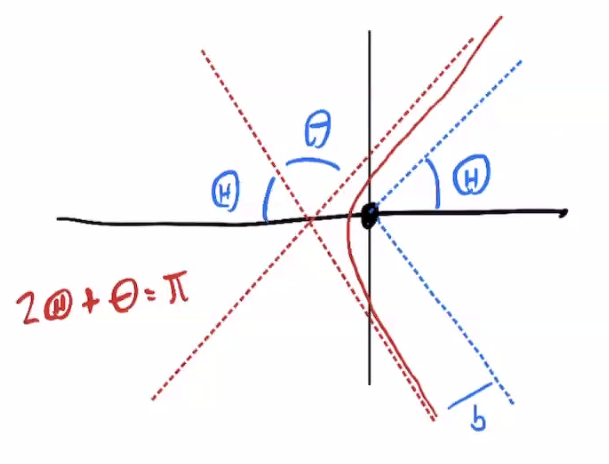
\includegraphics[scale = 0.3]{scattering.png}
\end{center}
we obtain 
\[2\Theta + \theta = \pi\]
The energy is given
\[E = \frac{1}{2}\mu v^2\]
and the angular momentum by
\[\ell = \abs{r\times p} = \mu v b\]
so we can substitute in to obtain
\[\theta(b) = \pi - 2\pi \int_{r_0}^\infty \frac{\d{r}}{r^2\sqrt{1-\frac{v(r)}{E - \frac{b^2}{r^2}}}}\]
where \(r_0\) is the distance of closest approach. Once we obtain \(\theta(b)\), we can compute \(\sigma(\theta)\) and compare to experiment.
\subsubsection{Rutherford Scattering}
While it is possible to use the previously derived equations to derive Rutherford scattering fromt the force, we can instead recognize that the potential is of the same form as gravity, and so we can use our trajectories we have previously derived. We can start from
\[U = -\frac{\alpha}{r}\]
\[E = \frac{1}{2}\mu r^2\]
\[\ell = \mu vb\]
\[2\Theta + \theta = \pi\]
\[e = \sqrt{1+\frac{2E\ell^2}{\mu \alpha^2}}\]
for hyperbolic orbits, we must further have
\[e \cos\Theta = 1\]
Using these equations, we can show
\[b(\theta = \frac{\alpha}{\mu v^2}\cot\frac{\theta}{2}\]
\[\sigma(\theta) = \frac{\alpha^2}{4\mu^2 v^2}*\frac{1}{\cos^4\theta/2}\]
